\begin{SCfigure}
  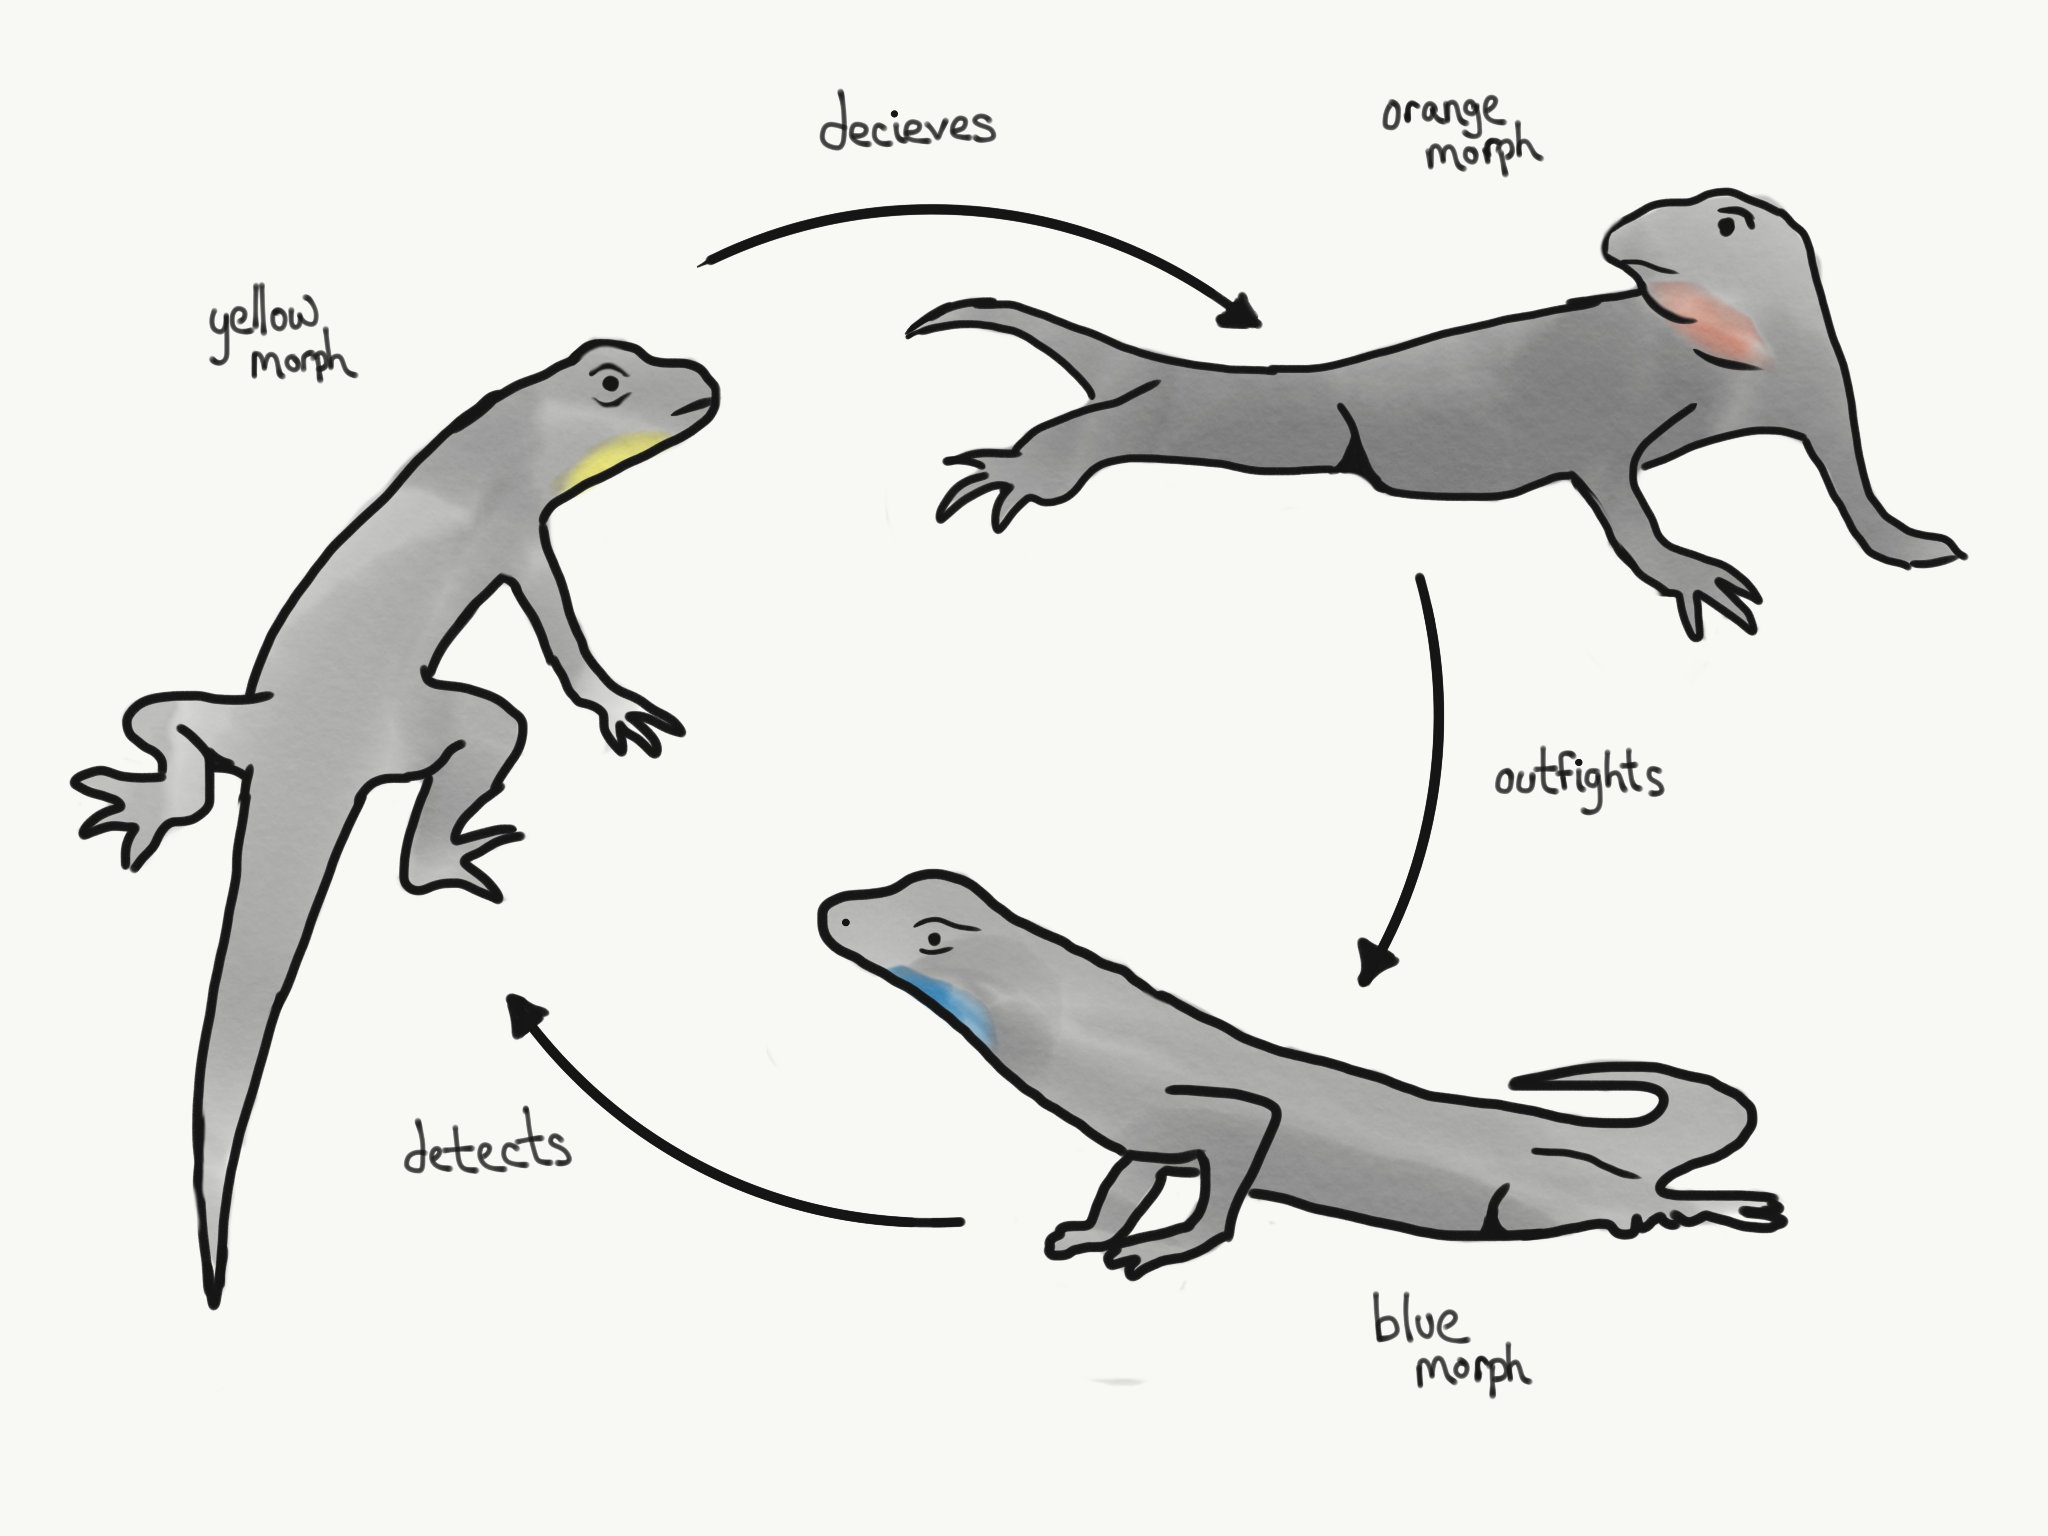
\includegraphics[width=0.7\textwidth]{img/lizards}
  %\captionsetup{singlelinecheck=off,justification=raggedright}
  \caption{The three male morphs of \textit{Uta stansburiana}, which exhibit different throat coloration and mating strategies, are shown to illustrate fitness degeneracy. Arrows indicate outcompetition for mates.\cite{Sinervo1996TheStrategies}.}
  \label{fig:spea_multiplicata}
\end{SCfigure}